\section{On-demand evaluation for KBP}
\label{sec:application}
Applying the on-demand evaluation framework to a task requires us to define three operations:
\begin{enumerate}
  \item How are instances sampled \pl{wouldn't use word sampled here - this is not about estimation but defining the objective function - say weighing instead} from a system's predictions, i.e.\ what is $p_i(x)$?
  \item How do we label an instance $x$, i.e.\ check if $x \in \sY$?
  \item How do we sample from the unknown set of true instances $x \sim \sY$?
\end{enumerate}
In this section, we'll present practical implementations for each of these operations for knowledge base population.

\subsection{Sampling from system predictions}
% 1. what is the point of this distribution?
% - prevent over sampling instances.
Recall that a KBP system predicts a set of relation instances of the form (\entity{subject}, \relation{predicate}, \entity{object}, \textsc{provenance}).
In practice, it is common for a system's predictions
to be be dominated by a few common predicates (e.g.\ professional titles) or
subject entities (e.g.\ ``United States of America'').
Thus, if we let $p_i$ be the uniform distribution over this set,
our evaluation metrics would be skewed towards a particular predicate or entity.
%The choice of distribution over this set determines how much we put weight on rare predicates and subject entities in our evaluation metric. % in our precision score. % PL: for recall 
We therefore propose two instance distributions that evaluate precision and recall scores macro-averaged over predicates and subject entities, respectively:
\begin{align*}
  p_i^\text{(p)}(x) &\eqdef \frac{1}{|\text{npreds}(X_i)|} \frac{1}{\operatorname{ninsts}(X_i, \relation{pred}(x))} \\
  p_i^\text{(e)}(x) &\eqdef \frac{1}{|\text{nsubjs}(X_i)|} \frac{1}{\operatorname{ninsts}(X_i, \relation{subj}(x))},
\end{align*}
where npreds, nsubjs specifies the number of predicates, subject entities in $X_i$ respectively  and ninsts the number of instances with the given predicate or subject entity.
See \refapp{implementation} for more details.

\begin{figure*}[t]
\begin{subfigure}{0.49\textwidth}
  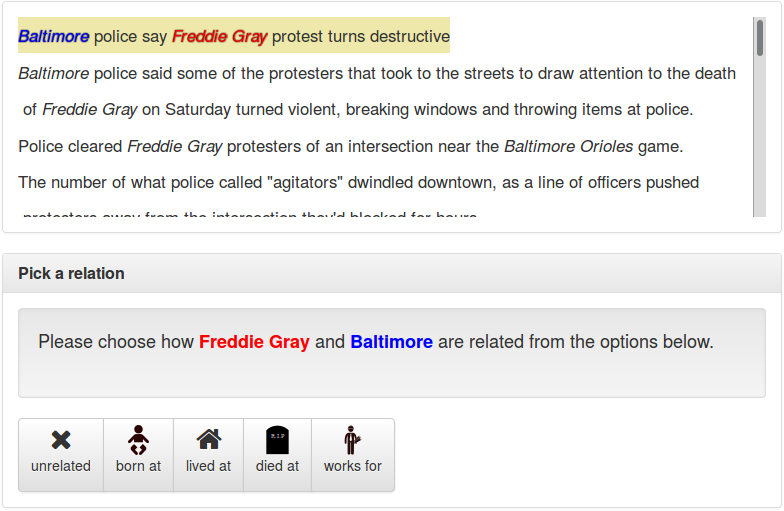
\includegraphics[width=\textwidth]{figures/interface/relation-interface}
  \caption{\label{fig:relation-interface} Relation extraction.}
\end{subfigure}
\hfill
\begin{subfigure}{0.49\textwidth}
  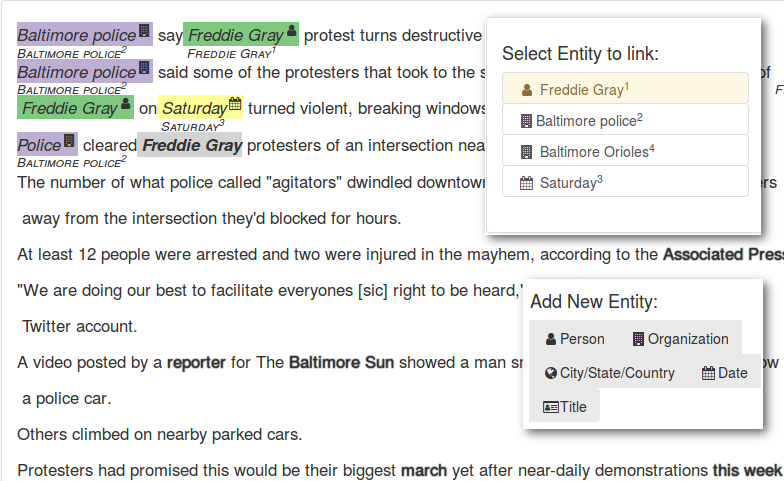
\includegraphics[width=\textwidth]{figures/interface/extraction-interface}
  \caption{\label{fig:entity-interface} Entity detection and linking.}
\end{subfigure}
\caption{\label{fig:interfaces} Interfaces for exhaustively annotating documents with its relation instances.}
\end{figure*}

\subsection{Labeling predicted instances}
We label predicted relation instances by presenting the instance's provenance to crowdworkers
  and asking them to identify if a relation holds between the identified subject and object mentions (\reffig{relation-interface}). 
  Crowd workers are also asked to link the subject and object mentions to their canonical mentions \ap{undefined} within the document and to pages on Wikipedia, if possible, for entity linking.
On average, we find that crowdworkers are able to perform this task in about 20 seconds, corresponding to about \$0.05 per instance.
We requested 5 crowdworkers to annotate a small set of 200 relation instances from the 2015 TAC-KBP corpus 
and measured a substantial inter-annotator agreement of 0.90 with 3 crowdworkers and 0.95 with 5 \pl{why does it go up with more annotators?}.
Consequently, we take a majority vote over 3 workers in subsequent experiments,
leading to a total cost of \$0.15 per relation instance.
%\pl{what does it mean to annotate a relation - get all the relation instances for that relation or just one?}.

\subsection{Sampling true instances}
Sampling from the set of true instances $\sY$ is difficult because we can't even enumerate the elements of $\sY$.
As a proxy, we assume that relations are identically distributed across documents and have crowdworkers annotate a random subset of documents for relations using an interface we developed (\reffig{entity-interface}).
Crowd workers begin by identifying every mention span in a document.
  For each mention, they are asked to identify its type, canonical mention within the document
  and associated Wikipedia page if possible.
They are then presented with a separate interface to label predicates between pairs of mentions within a sentence that were identified earlier.

We compare crowdsourced annotations against those of expert annotators using data from the TAC KBP 2015 EDL task on 10 randomly chosen documents.
We find that 3 crowdworkers together identify 92\% of the entity spans identified by expert annotators, while 7 crowdworkers together identify 96\%.
When using a token-level majority vote to identify entities, 3 crowdworkers identify about 78\% of the entity spans; this number does not change significantly with additional crowdworkers.
We also measure substantial token-level inter-annotator agreement for identifying typed mention spans ($\kappa = 0.83$), canonical mentions ($\kappa = 0.75$) and entity links ($\kappa = 0.75$) with just three workers.
Based on this analysis, we use token-level majority over 3 workers in subsequent experiments.

The entity annotation interface is far more involved and takes on average about 13 minutes per document, corresponding to about \$2.60 per document, while the relation annotation interface takes on average about \$2.25 per document.
Because documents vary significantly in length and complexity, we set rewards for each document based on the number of tokens (.75c per token) and mention pairs (5c per pair) respectively.
With 3 workers per document, we paid on average about \$15 per document.
On average, each document contained 9.2 relations and it cost about \$1.61 per relation, which is about ten times as much as labeling a relation.

A final issue to discuss is how documents themselves should be weighted to capture diverse entities that span documents; see \refapp{implementation} for details.
%We provide details regarding our sampling scheme and its distribution over entities in \refapp{implementation} of the supplementary material.
%When considering uniformly sampled documents, we found that a majority of the relations extracted correspond to very rare entities and result in very few entities with more than one relation (\reffig{entity-distribution}).
%In contrast, the TAC KBP query are almost evenly split between rare and semi-frequent entities.
%As a heuristic, we adopt the following two-stage sampling procedure:
%First, 20\% of our exhaustive document collection is sampled uniformly and annotated.
%We then uniformly sample the entities annotated to create a collection of ``query entities''.
%Finally, we construct the remaining 80\% of our document collection by searching for documents that contain the query entities according to an exact string match. This process results in far more entities of medium frequency.
